\section{Results}
\label{sec:results}

Unless stated, differences are paired by seed over 10 seeds with 95\% bootstrap intervals; the complete list of
hypotheses and verdicts is Table~\ref{tab:score}. Where a result contradicts a design claim we say so in the section where it appears.

\subsection{Trust establishment and cold start (E-CS1)}
\label{sec:res-cs1}
Table~\ref{tab:cs1} gives, per substrate, the simulated time to establish a donation session and the start latency from each
level of the warm-state ladder. Two facts shape everything that follows. First, the appliance pays a large \emph{one-off}
cost per session (\SimApplSession\,s with the pre-measurement parameters; \CalAttested\,s measured end to end on the
laptop), against \SimCvmSession\,s for a confidential VM and \SimCocoSession\,s for a confidential-container pool: trust on the appliance
is expensive to establish and everything is lost when the session ends. Second, once the session exists the appliance is as fast as
an unattested Firecracker host: warm and snapshot starts are within a few percent of the unattested figures (H5, supported), because
attestation is paid per session rather than per invocation. Confidential VMs invert the trade: cheap sessions but slower
lower ladder levels (Table~\ref{tab:cs1}). Our
a-priori expectation that confidential-VM classes establish trust 10--100$\times$ \emph{slower} than the appliance is refuted:
they are about 93\% faster, because the appliance's cost is a reboot. Measurements on the laptop agree with the simulated
ladder: a warm Firecracker start takes \CalFcBootWarmMs\,ms, a cold-cache boot \CalFcBootColdS\,s, and creating a 512\,MB
snapshot \CalSnapCreate\,s on a hard disk, which makes snapshots something to plan rather than to take on demand.

\begin{table}[t]
\caption{Simulated session establishment and start latency (s) from each warm-state level (L0 nothing cached, L3 warm idle
VM; ``--'' not applicable). Pre-measurement parameters (Table~\ref{tab:calib}).}
\label{tab:cs1}
\centering\scriptsize
\resizebox{\columnwidth}{!}{% Generated by experiments/paper_tex.py; do not edit.
\begin{tabular}{lrrrrr}
\toprule
\textbf{Substrate} & \textbf{Session} & \textbf{L0} & \textbf{L1} & \textbf{L2} & \textbf{L3} \\
\midrule

appliance (TPM) & 19.2 & 1.45 & 0.346 & 0.0285 & 0.00197 \\
DRTM hypervisor & 2.31 & 1.44 & 0.34 & 0.0284 & 0.00196 \\
CVM (SEV-SNP) & 1.41 & 2.31 & 1.19 & 0.155 & 0.002 \\
CoCo pool & 8.11 & 2.25 & 1.14 & -- & 0.002 \\
no attestation & 1.06 & 1.45 & 0.344 & 0.0278 & 0.00201 \\
\bottomrule
\end{tabular}
}
\end{table}

\subsection{Where is the system viable? (E20)}
\label{sec:res-viab}
Averages hide the regimes in which a design fails, so we map viability (Sec.~\ref{sec:method}) over three two-dimensional
panels. Figure~\ref{fig:viab} colors each cell by which system is viable under the default criterion (success $\ge0.99$ and deadline-met $\ge0.95$) and prints \voss{}'s P99.
Table~\ref{tab:viab} counts \voss{}-viable cells under other targets.

\begin{figure*}[t]
\centering
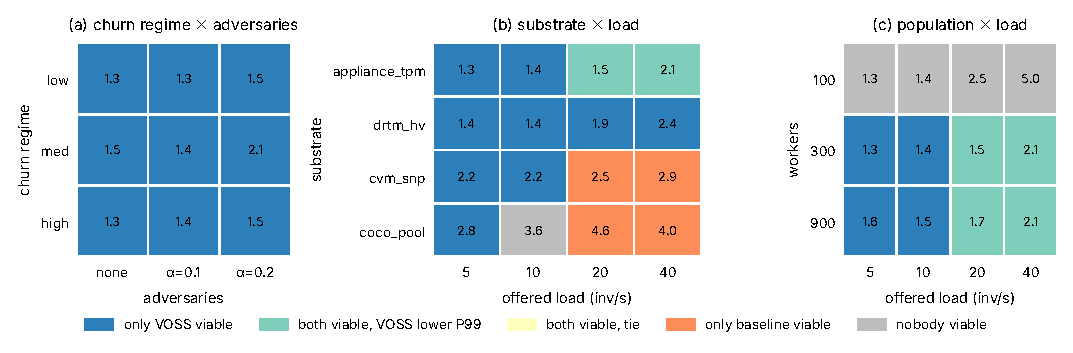
\includegraphics[width=\textwidth]{figures/fig_viability}
\caption{Viability maps (E20). Cell color: which of \voss{} and the best simple baseline is viable (success $\ge0.99$,
deadline-met $\ge0.95$); numbers: \voss{} sync P99 in seconds. (a) churn regime against adversary fraction, (b) substrate against offered load (inv/s),
(c) population against offered load.}
\label{fig:viab}
\end{figure*}

\begin{table}[t]
\caption{Number of cells in which \voss{} is viable, by target (deadline-met fraction, or absolute sync P99).}
\label{tab:viab}
\centering\scriptsize
\resizebox{\columnwidth}{!}{% Generated by experiments/paper_tex.py; do not edit.
\begin{tabular}{lrrrrrrr}
\toprule
\textbf{Panel} & \textbf{0.90} & \textbf{0.95} & \textbf{0.98} & \textbf{2 s} & \textbf{3 s} & \textbf{5 s} & \textbf{Cells} \\
\midrule
& \multicolumn{3}{c}{deadline-met target} & \multicolumn{3}{c}{sync P99 target} & \\
\cmidrule(lr){2-4}\cmidrule(lr){5-7}
A: churn $\times$ $\alpha$ & 9 & 9 & 0 & 8 & 9 & 9 & 9 \\
B: substrate $\times$ load & 16 & 11 & 0 & 6 & 13 & 16 & 16 \\
C: $N$ $\times$ load & 8 & 8 & 0 & 8 & 10 & 10 & 12 \\
\bottomrule
\end{tabular}
}
\end{table}

\voss{} is the \emph{only} viable system in all \ViabACells{} cells of panel A, which spans three churn regimes and up to $20\%$ omitting owners, in
\ViabBMetOnly{} of \ViabBCells{} cells of panel B and in \ViabCMetOnly{} of \ViabCCells{} cells of panel C. With an absolute sync P99 target of 3\,s
it is viable in \ViabAPThreeVoss{} of \ViabACells, \ViabBPThreeVoss{} of \ViabBCells{} and \ViabCPThreeVoss{} of \ViabCCells{} cells, and the simple baseline in none of them; at
5\,s \voss{} is viable in \ViabAPFiveVoss, \ViabBPFiveVoss{} and \ViabCPFiveVoss{} cells. The two criteria measure different things (a deadline is a multiple of the
warm latency; the absolute target is what a user perceives), which is why a baseline can pass one and fail the other.

The map also shows where \voss{} is \emph{not} the right choice. On confidential-VM and confidential-container substrates at higher load, the simple baseline
is the only viable system in \ViabBMetBase{} cells (Fig.~\ref{fig:viab}b): we conjecture that with cheap session establishment there is little cold-start cost for planning to remove, while it still adds exposure and memory;
we did not test this. With 100 workers no system is viable in any cell of panel C
(\ViabCMetNoneFive{} cells), so the design needs a minimum population, and at a deadline-met target of 0.98 \emph{no} system is viable in any cell: the
``98\% of sync invocations within $5\times$ warm latency'' service level is out of reach in this setting for \voss{} and the baselines alike.

\subsection{Planning trust and warm state (E04, E19)}
\label{sec:res-plan}
Table~\ref{tab:plan} compares planners on the same scenarios under medium and high churn. Planning is the largest single lever: the robust MILP
cuts sync P99 by \HOnePctNoneMed\% (medium churn) and \HOnePctNoneHigh\% (high churn) against no planning, and by \HOnePctKeepMed\% and
\HOnePctKeepHigh\% against a keep-alive TTL (H1, supported). It pays with donor memory: about \MilpWarmRatio$\times$ the warm memory of
keep-alive at medium churn. The comparison that
motivates the integer program is weaker. The MILP is only \HEightPct\% better than the greedy planner at high churn (H8, interval includes
zero, inconclusive) while its solve time is \MilpSolveS\,s per cluster against \GreedySolveMs\,ms. We cannot, on this evidence, claim that the
exact solver pays for itself. What it gives, beyond latency, is the coverage guarantee of Eq.~\eqref{eq:robust}, whose value is shown below.

\begin{table}[t]
\caption{Planner comparison (E04): mean $\pm$ 95\% half-width over 10 seeds. Met: deadline-met fraction; Warm: GB of idle warm memory.}
\label{tab:plan}
\centering\scriptsize
\resizebox{\columnwidth}{!}{% Generated by experiments/paper_tex.py; do not edit.
\begin{tabular}{llrrrrr}
\toprule
\textbf{Regime} & \textbf{Planner} & \textbf{P99 (s)} & \textbf{Met} & \textbf{Warm GB} & \textbf{Exposure} & \textbf{Solve (s)} \\
\midrule

churn\_med & no planning & 2.78{\scriptsize$\pm$1.35} & 0.940{\scriptsize$\pm$0.017} & 1{\scriptsize$\pm$0} & 8.5{\scriptsize$\pm$1.4} & 0.001{\scriptsize$\pm$0.000} \\
churn\_med & keep-alive TTL & 1.78{\scriptsize$\pm$0.48} & 0.971{\scriptsize$\pm$0.018} & 61{\scriptsize$\pm$9} & 7.4{\scriptsize$\pm$1.1} & 0.002{\scriptsize$\pm$0.001} \\
churn\_med & greedy planner & 1.29{\scriptsize$\pm$0.09} & 0.978{\scriptsize$\pm$0.015} & 94{\scriptsize$\pm$14} & 19.9{\scriptsize$\pm$1.8} & 0.005{\scriptsize$\pm$0.000} \\
churn\_med & robust MILP & 1.26{\scriptsize$\pm$0.11} & 0.979{\scriptsize$\pm$0.014} & 131{\scriptsize$\pm$19} & 20.1{\scriptsize$\pm$1.7} & 3.333{\scriptsize$\pm$0.457} \\
churn\_high & no planning & 3.48{\scriptsize$\pm$1.32} & 0.923{\scriptsize$\pm$0.029} & 1{\scriptsize$\pm$0} & 7.5{\scriptsize$\pm$1.2} & 0.001{\scriptsize$\pm$0.000} \\
churn\_high & keep-alive TTL & 3.28{\scriptsize$\pm$1.91} & 0.940{\scriptsize$\pm$0.030} & 59{\scriptsize$\pm$10} & 7.3{\scriptsize$\pm$0.9} & 0.001{\scriptsize$\pm$0.000} \\
churn\_high & greedy planner & 1.42{\scriptsize$\pm$0.17} & 0.958{\scriptsize$\pm$0.028} & 87{\scriptsize$\pm$13} & 15.8{\scriptsize$\pm$1.2} & 0.006{\scriptsize$\pm$0.001} \\
churn\_high & robust MILP & 1.38{\scriptsize$\pm$0.16} & 0.959{\scriptsize$\pm$0.031} & 115{\scriptsize$\pm$12} & 15.0{\scriptsize$\pm$0.8} & 3.291{\scriptsize$\pm$0.502} \\
\bottomrule
\end{tabular}
}
\end{table}

Figure~\ref{fig:abl} removes one component of \voss{} at a time (E19). Removing lifecycle-aware placement costs
\AblLifecycleP\,s of sync P99, removing planning \AblPlanningP\,s (and lowers exposure by \AblPlanningExp, because less is pre-warmed and fewer hosts hold keys), removing the robust
constraint \AblRobustP\,s (exposure \AblRobustExp{} lower) and removing hedging \AblHedgeP\,s. Geo-clustering is the only component whose removal
\emph{improves} P99 (\AblGeoP\,s lower), and it also cuts exposure by \AblGeoExp: Sec.~\ref{sec:res-geo}. Putting reputation into the cost matrix instead of using it
as a tie-breaker raises exposure by \AblRepExp. The ablations also show where trust and latency trade against each other: the same components that buy P99
(planning, robustness) raise exposure.

\begin{figure}[t]
\centering
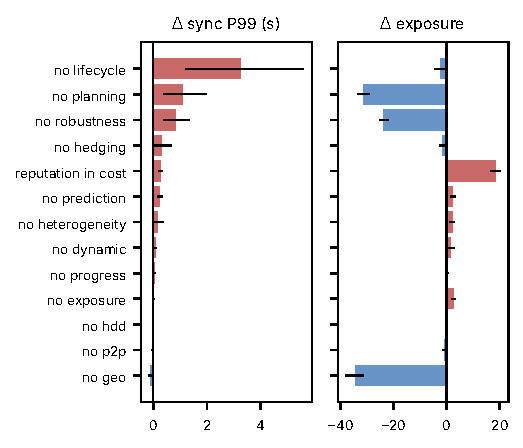
\includegraphics[width=\columnwidth]{figures/fig_ablation}
\caption{Ablations (E19): change when a component is removed, relative to full \voss{} (paired, 95\% intervals).
Left: sync P99; right: key-holder exposure.}
\label{fig:abl}
\end{figure}

\subsection{Faults, adversaries and the latency--exposure trade-off (E08, E15, E16, E23)}
\label{sec:res-ft}

\medskip\noindent\textbf{Detection.}
Table~\ref{tab:faults} injects crashes, partitions, black-holing and slowed scheduler hosts. Heartbeats alone cannot see a black hole: the
host keeps sending liveness while dropping work, so detection waits for the 60\,s timeout (\BhDetectHb\,s) and the run suffers \BhTimeoutsHb{} timeouts, against
\BhDetectProg\,s and \BhTimeoutsProg{} with progress-based detection (H-FT1, supported). For plain crashes progress detection needs \CrashDetectProg\,s and
failover \CrashFailover\,s. A slowed-but-live scheduler is the hardest case: failover takes \SlowFailover\,s on average because progress evidence must
accumulate before the slowdown is distinguishable from load.

\begin{table}[t]
\caption{Scheduler faults (E15): time to detection, failover, success and P99 within the fault window.}
\label{tab:faults}
\centering\scriptsize
\resizebox{\columnwidth}{!}{% Generated by experiments/paper_tex.py; do not edit.
\begin{tabular}{llrrrr}
\toprule
\textbf{Fault} & \textbf{Detector} & \textbf{Detect (s)} & \textbf{Failover (s)} & \textbf{Success (\%)} & \textbf{P99 in window (s)} \\
\midrule

crash & progress & 2.2{\scriptsize$\pm$0.3} & 2.7{\scriptsize$\pm$0.4} & 99.95{\scriptsize$\pm$0.02} & 1.28{\scriptsize$\pm$0.15} \\
crash & heartbeat\_only & 5.0{\scriptsize$\pm$0.0} & 5.5{\scriptsize$\pm$0.5} & 99.87{\scriptsize$\pm$0.04} & 1.66{\scriptsize$\pm$0.33} \\
partition & progress & 2.2{\scriptsize$\pm$0.3} & 2.6{\scriptsize$\pm$0.4} & 99.95{\scriptsize$\pm$0.02} & 1.28{\scriptsize$\pm$0.16} \\
partition & heartbeat\_only & 5.0{\scriptsize$\pm$0.0} & 5.5{\scriptsize$\pm$0.5} & 99.87{\scriptsize$\pm$0.04} & 1.67{\scriptsize$\pm$0.31} \\
blackhole & progress & 4.2{\scriptsize$\pm$3.0} & 4.6{\scriptsize$\pm$3.0} & 99.95{\scriptsize$\pm$0.02} & 1.28{\scriptsize$\pm$0.15} \\
blackhole & heartbeat\_only & 60.0{\scriptsize$\pm$0.0} & 59.3{\scriptsize$\pm$1.1} & 96.81{\scriptsize$\pm$0.51} & 2.90{\scriptsize$\pm$0.08} \\
slow & progress & 13.9{\scriptsize$\pm$7.9} & 14.3{\scriptsize$\pm$8.2} & 99.95{\scriptsize$\pm$0.03} & 1.34{\scriptsize$\pm$0.14} \\
slow & heartbeat\_only & 60.0{\scriptsize$\pm$0.0} & 59.3{\scriptsize$\pm$1.1} & 99.55{\scriptsize$\pm$0.41} & 2.00{\scriptsize$\pm$0.33} \\
\bottomrule
\end{tabular}
}
\end{table}

\medskip\noindent\textbf{Omitting owners.}
Table~\ref{tab:adv} sweeps the fraction $\alpha$ of omitting owners. With $\alpha=0.2$ \voss{} keeps success at \VossSuccAlpha\%, whereas
heartbeat-only detection with otherwise identical machinery drops to \HbSuccAlpha\% (H4, supported). Progress detection also gives
\HbOmitRatio$\times$ fewer results dropped by omitting owners at $\alpha=0.2$. The hypothesis that the \emph{robust} planning constraint is what keeps success
is not supported: setting $f=0$ changes success by only \FzeroSuccDelta{} percentage points (H2, inconclusive), though it lengthens P99 (Table~\ref{tab:adv}).
Detection and re-dispatch, not redundant coverage, carry the success; robust planning buys tail latency.

\begin{table}[t]
\caption{Omitting owners (E08), mean $\pm$ 95\% half-width over 10 seeds. Omissions: results dropped by adversaries.}
\label{tab:adv}
\centering\scriptsize
\resizebox{\columnwidth}{!}{% Generated by experiments/paper_tex.py; do not edit.
\begin{tabular}{llrrrr}
\toprule
\textbf{Adversaries} & \textbf{System} & \textbf{Success (\%)} & \textbf{P99 (s)} & \textbf{Waste (\%)} & \textbf{Omissions} \\
\midrule

none $\alpha$=0 & VOSS & 99.99{\scriptsize$\pm$0.01} & 1.27{\scriptsize$\pm$0.11} & 1.7{\scriptsize$\pm$0.5} & 0{\scriptsize$\pm$0} \\
none $\alpha$=0 & VOSS, $f{=}0$ & 99.99{\scriptsize$\pm$0.01} & 1.60{\scriptsize$\pm$0.24} & 2.2{\scriptsize$\pm$0.6} & 0{\scriptsize$\pm$0} \\
none $\alpha$=0 & heartbeat-only & 99.98{\scriptsize$\pm$0.01} & 1.36{\scriptsize$\pm$0.15} & 2.0{\scriptsize$\pm$0.7} & 0{\scriptsize$\pm$0} \\
mixed $\alpha$=0.1 & VOSS & 99.95{\scriptsize$\pm$0.04} & 1.32{\scriptsize$\pm$0.12} & 2.2{\scriptsize$\pm$0.5} & 38{\scriptsize$\pm$14} \\
mixed $\alpha$=0.1 & VOSS, $f{=}0$ & 99.96{\scriptsize$\pm$0.03} & 2.15{\scriptsize$\pm$0.60} & 2.9{\scriptsize$\pm$0.6} & 37{\scriptsize$\pm$11} \\
mixed $\alpha$=0.1 & heartbeat-only & 98.19{\scriptsize$\pm$0.75} & 1.36{\scriptsize$\pm$0.13} & 4.0{\scriptsize$\pm$0.9} & 298{\scriptsize$\pm$115} \\
mixed $\alpha$=0.2 & VOSS & 99.95{\scriptsize$\pm$0.03} & 1.43{\scriptsize$\pm$0.16} & 2.6{\scriptsize$\pm$0.5} & 61{\scriptsize$\pm$13} \\
mixed $\alpha$=0.2 & VOSS, $f{=}0$ & 99.83{\scriptsize$\pm$0.17} & 2.05{\scriptsize$\pm$0.52} & 3.5{\scriptsize$\pm$0.8} & 80{\scriptsize$\pm$31} \\
mixed $\alpha$=0.2 & heartbeat-only & 96.79{\scriptsize$\pm$1.13} & 1.39{\scriptsize$\pm$0.16} & 5.6{\scriptsize$\pm$1.3} & 527{\scriptsize$\pm$161} \\
all $\alpha$=0.2 & VOSS & 99.94{\scriptsize$\pm$0.05} & 1.37{\scriptsize$\pm$0.10} & 2.3{\scriptsize$\pm$0.7} & 31{\scriptsize$\pm$9} \\
all $\alpha$=0.2 & VOSS, $f{=}0$ & 99.96{\scriptsize$\pm$0.03} & 2.28{\scriptsize$\pm$1.00} & 2.7{\scriptsize$\pm$0.5} & 28{\scriptsize$\pm$8} \\
all $\alpha$=0.2 & heartbeat-only & 97.70{\scriptsize$\pm$1.26} & 1.42{\scriptsize$\pm$0.14} & 5.2{\scriptsize$\pm$2.4} & 385{\scriptsize$\pm$227} \\
\bottomrule
\end{tabular}
}
\end{table}

\medskip\noindent\textbf{Hedging.}
Hedging duplicates risky invocations. Always hedging cuts P99 but wastes \AlwaysWastePct\% extra attempts. Risk-proportional hedging (hedge with probability
tied to estimated risk, within a 5\% budget) wastes \RpWastePct\%, and its P99 is \HedgePNinetyninePct\% lower with $\alpha=0.1$ but with an interval from
\HedgePNinetynineLo\% to $+$\HedgePNinetynineHi\% (H-FT3, inconclusive). It is cheap insurance, not demonstrated to be necessary.

\medskip\noindent\textbf{Pareto front.}
Robustness $f$ and the exposure weight trade latency against key-holder exposure (E23, Fig.~\ref{fig:pareto}). The aggregate front has \ParetoFrontN{}
points. Exposure grows with $f$ (\ExpFZero, \ExpFOne{} and \ExpFTwo{} at $f=0$, $0.1$, $0.2$), consistent with covering any $f$ failures requiring more key-holding hosts. Aggregate sync P99 stays
within \ParetoPNinetynineLo--\ParetoPNinetynineHi\,s across configurations, so the knee at $f=\ParetoKneeF$ saves \ParetoKneeExpSaved\% of exposure against the best-latency front point for
\ParetoKneePNinetynineLoss\% more P99 (H3, supported): moderate exposure budgets are cheap. Per tenant class the picture is less benign. Low-sensitivity tenants stay at about \ParetoLowMax\,s or below, but for
high-sensitivity tenants P99 reaches \ParetoHighMax\,s in one robust configuration, while an $f=0$ configuration has the lowest exposure at nearly the best P99. The aggregate knee therefore should not be applied to every class;
sensitivity classes need their own operating point.

\begin{figure}[t]
\centering
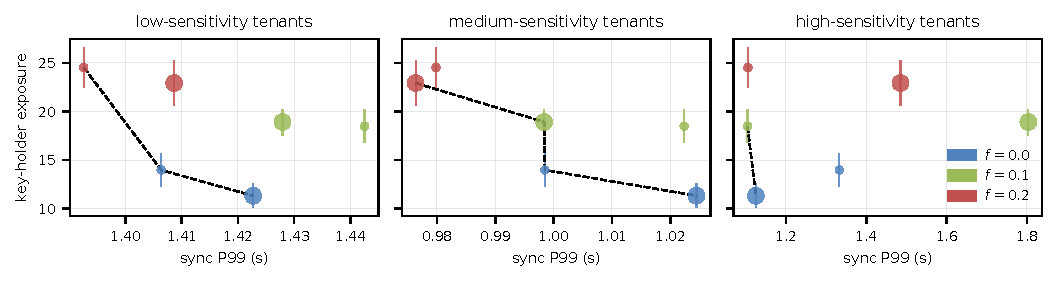
\includegraphics[width=\columnwidth]{figures/fig_pareto}
\caption{Latency--exposure--robustness (E23). Each point is a ($f$, exposure weight) configuration (marker size: weight) with 95\% error bars on exposure;
the dashed line is the Pareto front per tenant sensitivity class.}
\label{fig:pareto}
\end{figure}

\subsection{Geography, routing and caching (E05--E07, E09)}
\label{sec:res-geo}
The geographic hierarchy, a central idea of the design, does not pay off at the scale we simulate. Table~\ref{tab:geo} compares a single global scheduler
against static regions, static $k$-means and dynamic clusters. Dynamic clusters have \emph{higher} P99 than the global scheduler by
\HSevenEu\% (Europe), \HSevenEuNa\% (EU+NA) and \HSevenWorld\% (world) (H7, refuted at all three populations), and hold \GeoExpRatio$\times$ the key-holder
exposure in Europe, since each of the \GeoClusters{} clusters must cover demand with its own key holders. The network share of latency
does fall in some populations (Table~\ref{tab:geo}), but not enough to offset the cost of splitting the pool. We attribute this to fewer hosts per
cluster for pooling warm state and keys, but did not isolate the mechanism. Our results show no population in which geo-clustering wins at the scale we simulate.

\begin{table}[t]
\caption{Geo-clustering (E05): mean $\pm$ 95\% half-width over 10 seeds.}
\label{tab:geo}
\centering\scriptsize
\resizebox{\columnwidth}{!}{% Generated by experiments/paper_tex.py; do not edit.
\begin{tabular}{llrrrr}
\toprule
\textbf{Population} & \textbf{Clustering} & \textbf{P99 (s)} & \textbf{Network (s)} & \textbf{Clusters} & \textbf{Exposure} \\
\midrule

Europe & one global scheduler & 1.06{\scriptsize$\pm$0.09} & 0.092{\scriptsize$\pm$0.015} & 1.0{\scriptsize$\pm$0.0} & 12{\scriptsize$\pm$1} \\
Europe & static regions & 1.06{\scriptsize$\pm$0.09} & 0.092{\scriptsize$\pm$0.015} & 1.0{\scriptsize$\pm$0.0} & 12{\scriptsize$\pm$1} \\
Europe & static $k$-means & 1.25{\scriptsize$\pm$0.09} & 0.124{\scriptsize$\pm$0.031} & 10.4{\scriptsize$\pm$0.5} & 63{\scriptsize$\pm$4} \\
Europe & dynamic & 1.24{\scriptsize$\pm$0.10} & 0.127{\scriptsize$\pm$0.037} & 9.1{\scriptsize$\pm$0.6} & 61{\scriptsize$\pm$4} \\
EU + NA & one global scheduler & 1.14{\scriptsize$\pm$0.09} & 0.154{\scriptsize$\pm$0.021} & 1.0{\scriptsize$\pm$0.0} & 14{\scriptsize$\pm$1} \\
EU + NA & static regions & 1.20{\scriptsize$\pm$0.13} & 0.123{\scriptsize$\pm$0.014} & 2.0{\scriptsize$\pm$0.0} & 24{\scriptsize$\pm$2} \\
EU + NA & static $k$-means & 1.31{\scriptsize$\pm$0.13} & 0.151{\scriptsize$\pm$0.031} & 7.5{\scriptsize$\pm$0.4} & 54{\scriptsize$\pm$3} \\
EU + NA & dynamic & 1.33{\scriptsize$\pm$0.20} & 0.127{\scriptsize$\pm$0.013} & 6.4{\scriptsize$\pm$0.6} & 52{\scriptsize$\pm$4} \\
world & one global scheduler & 1.21{\scriptsize$\pm$0.11} & 0.192{\scriptsize$\pm$0.016} & 1.0{\scriptsize$\pm$0.0} & 13{\scriptsize$\pm$1} \\
world & static regions & 1.36{\scriptsize$\pm$0.12} & 0.167{\scriptsize$\pm$0.013} & 6.6{\scriptsize$\pm$0.3} & 43{\scriptsize$\pm$4} \\
world & static $k$-means & 1.31{\scriptsize$\pm$0.11} & 0.164{\scriptsize$\pm$0.020} & 7.0{\scriptsize$\pm$0.5} & 48{\scriptsize$\pm$3} \\
world & dynamic & 1.27{\scriptsize$\pm$0.11} & 0.157{\scriptsize$\pm$0.018} & 6.0{\scriptsize$\pm$0.3} & 46{\scriptsize$\pm$3} \\
\bottomrule
\end{tabular}
}
\end{table}

Routing matters more than clustering. Without flash crowds, nearest-region routing meets \RouteNearMet{} of deadlines (P99 \RouteNearPNinetynine\,s),
whereas routing to the least-loaded cluster meets \RouteLeastMet{} (P99 \RouteLeastPNinetynine\,s) because it ignores distance. Spilling to other clusters is rare and priced (E07).
For caching (E09) the cost-aware GDSF policy with peer-to-peer fetch and an HDD tier is at most \HSixPct\% better than LRU in sync P99
and the intervals include zero (H6, inconclusive). All variants start about 98\% of invocations from a warm VM, which leaves little for the disk tiers to improve.

\subsection{Is the machinery needed? Simple baseline and commercial references (E10, E17)}
\label{sec:res-simple}
Table~\ref{tab:simple} compares \voss{} with the simple baseline (least-loaded placement on the nearest attested worker, no planning). We expected the
baseline to match \voss{} on homogeneous, stable, benign hardware. It does not: \voss{} has \HElevenPct\% lower P99 (H11, refuted), even though
the pool is homogeneous; we attribute this to planning's pre-warming against churn, which the baseline lacks. The baseline, however, holds about half of \voss{}'s exposure (\voss{}
is \SimpleExpRatio$\times$ higher) consistent with its placing keys on fewer hosts. Whether the latency is worth the exposure is a
policy choice, and the E23 front (above) lets a deployer pick.

\begin{table}[t]
\caption{Simple baseline versus \voss{} (E10).}
\label{tab:simple}
\centering\scriptsize
\resizebox{\columnwidth}{!}{% Generated by experiments/paper_tex.py; do not edit.
\begin{tabular}{llrrr}
\toprule
\textbf{Hardware} & \textbf{System} & \textbf{P99 (s)} & \textbf{Met} & \textbf{Exposure} \\
\midrule

homogeneous & simple baseline & 3.90{\scriptsize$\pm$1.00} & 0.962{\scriptsize$\pm$0.012} & 64{\scriptsize$\pm$4} \\
homogeneous & VOSS & 2.38{\scriptsize$\pm$0.47} & 0.978{\scriptsize$\pm$0.007} & 122{\scriptsize$\pm$7} \\
mixed & simple baseline & 2.66{\scriptsize$\pm$0.24} & 0.969{\scriptsize$\pm$0.012} & 54{\scriptsize$\pm$3} \\
mixed & VOSS & 1.31{\scriptsize$\pm$0.09} & 0.989{\scriptsize$\pm$0.003} & 95{\scriptsize$\pm$4} \\
\bottomrule
\end{tabular}
}
\end{table}

Table~\ref{tab:comm} compares \voss{} with commercial-style references on the same workload and engine, priced with list prices. At 20\,inv/s
\voss{}'s P99 is \CommPNinetyninePct\% and its P50 \CommPFiftyPct\% above the Lambda-like reference, which uses always-on datacenter hosts. We attribute the gap to
perishable sandboxes and longer network paths on volunteer hardware. Cost per million invocations, including the
orchestrator tier but excluding volunteer credits, falls from \CommCostTen{} USD at 10\,inv/s through \CommCostTwenty{} to \CommCostForty{} at 40\,inv/s as the fixed tier is amortized,
against about \CommCostRef{} USD for the references. \voss{} is thus cost-competitive only above roughly 20\,inv/s on this workload, and it never has lower latency.

\begin{table}[t]
\caption{Commercial-style references versus \voss{} (E17). Met: deadline-met fraction; cost in USD per million invocations.}
\label{tab:comm}
\centering\scriptsize
\resizebox{\columnwidth}{!}{% Generated by experiments/paper_tex.py; do not edit.
\begin{tabular}{rlrrrr}
\toprule
\textbf{Load (inv/s)} & \textbf{System} & \textbf{P50 (s)} & \textbf{P99 (s)} & \textbf{Met} & \textbf{USD/M inv.} \\
\midrule

10 & VOSS & 0.425{\scriptsize$\pm$0.083} & 1.33{\scriptsize$\pm$0.08} & 0.987{\scriptsize$\pm$0.005} & 19.6{\scriptsize$\pm$0.9} \\
10 & Lambda-like & 0.292{\scriptsize$\pm$0.090} & 1.21{\scriptsize$\pm$0.12} & 0.999{\scriptsize$\pm$0.000} & 12.1{\scriptsize$\pm$4.5} \\
10 & Azure-like & 0.292{\scriptsize$\pm$0.090} & 1.33{\scriptsize$\pm$0.13} & 0.997{\scriptsize$\pm$0.000} & 12.0{\scriptsize$\pm$4.4} \\
20 & VOSS & 0.425{\scriptsize$\pm$0.082} & 1.27{\scriptsize$\pm$0.11} & 0.987{\scriptsize$\pm$0.006} & 9.8{\scriptsize$\pm$0.5} \\
20 & Lambda-like & 0.292{\scriptsize$\pm$0.090} & 1.11{\scriptsize$\pm$0.10} & 0.999{\scriptsize$\pm$0.000} & 12.1{\scriptsize$\pm$4.6} \\
20 & Azure-like & 0.292{\scriptsize$\pm$0.090} & 1.17{\scriptsize$\pm$0.11} & 0.998{\scriptsize$\pm$0.000} & 11.9{\scriptsize$\pm$4.4} \\
40 & VOSS & 0.442{\scriptsize$\pm$0.084} & 1.50{\scriptsize$\pm$0.23} & 0.979{\scriptsize$\pm$0.009} & 4.9{\scriptsize$\pm$0.2} \\
40 & Lambda-like & 0.292{\scriptsize$\pm$0.091} & 1.10{\scriptsize$\pm$0.10} & 0.999{\scriptsize$\pm$0.000} & 12.1{\scriptsize$\pm$4.6} \\
40 & Azure-like & 0.292{\scriptsize$\pm$0.090} & 1.15{\scriptsize$\pm$0.11} & 0.998{\scriptsize$\pm$0.000} & 11.9{\scriptsize$\pm$4.5} \\
\bottomrule
\end{tabular}
}
\end{table}

\subsection{Accounting and reputation (E12, E13)}
\label{sec:res-acct}
Attested receipts are off the critical path (H10, supported): lengthening the settlement period from 10 to 300\,s or the batch from 0.2 to 5\,s changes P99
by no more than $\pm$\HTenPct\%. The stream is small, about \RecvRows{} rows/s and \RecvKBs\,KB/s at 20\,inv/s offered load, every receipt is accounted for (\RecvUnexplained{} unexplained
receipts, at most \RecvMissingMax{} receipt missing at the end of a run) and verification costs \RecvVerifyMs\,ms per second. The settlement period sets the latency from receipt to credit:
\RecvLatTen, \RecvLatSixty{} and \RecvLatThreeHundred\,s for 10, 60 and 300\,s periods.
Reputation, however, adds little. Using a Beta-decay score only as a tie-breaker lowers P99 by \RepPNinetyninePct\% (E12, weak), and credit is highly concentrated: the Gini coefficient is
\RepGini, the top 10\% of workers earn \RepTopTen\% of credit and \RepStarved\% earn almost none, which is a fairness problem for an incentive that relies on credits.

\subsection{Scalability (E18)}
\label{sec:res-scale}
Figure~\ref{fig:scale} and Table~\ref{tab:scale} scale the population from $10^2$ to $10^5$ workers at constant load per worker (0.01\,inv/s) in a cheaper
``scalability mode'' (coarse heartbeats, greedy planning, 2 simulated minutes). Up to $10^4$ workers success is
\ScaleTenKSucc\%. At $3\times10^4$ it falls to \ScaleMidSucc\% with a decision P99 of \ScaleMidDecide\,s, and at $10^5$ to \ScaleBigSucc\% with sync P99 \ScaleBigPNinetynine\,s
and decision P99 \ScaleBigDecide\,s: decision latency grows from about 0.1\,s to tens of seconds. Per-worker control traffic stays flat
(\ScaleMsgLo--\ScaleMsgHi{} messages per second per worker), so the limit lies in the central decision path rather than in the message volume; we did not isolate
which orchestrator or router component saturates first, and the two largest points use three seeds. We read this as a measured limit of the current orchestrator tier, not of the approach.

\begin{figure}[t]
\centering
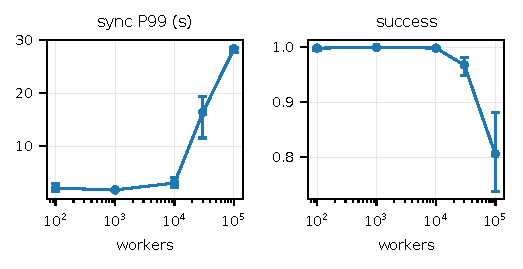
\includegraphics[width=\columnwidth]{figures/fig_scale}
\caption{Scalability (E18): sync P99 and success against population (log scale), mean with 95\% intervals; the two largest points use 3 seeds.}
\label{fig:scale}
\end{figure}

\begin{table}[t]
\caption{Scalability (E18): orchestrator and control-plane load.}
\label{tab:scale}
\centering\scriptsize
\resizebox{\columnwidth}{!}{% Generated by experiments/paper_tex.py; do not edit.
\begin{tabular}{rrrrrrr}
\toprule
\textbf{Workers} & \textbf{Seeds} & \textbf{Success (\%)} & \textbf{P99 (s)} & \textbf{Decide P99 (s)} & \textbf{Msg/s/worker} & \textbf{Orch. CPU (s/s)} \\
\midrule

100 & 10 & 99.8{\scriptsize$\pm$0.3} & 2.1{\scriptsize$\pm$0.8} & 0.10{\scriptsize$\pm$0.01} & 0.97{\scriptsize$\pm$0.04} & 0.000{\scriptsize$\pm$0.000} \\
1\,000 & 10 & 100.0{\scriptsize$\pm$0.1} & 1.7{\scriptsize$\pm$0.2} & 0.10{\scriptsize$\pm$0.01} & 0.74{\scriptsize$\pm$0.01} & 0.002{\scriptsize$\pm$0.000} \\
10\,000 & 10 & 99.8{\scriptsize$\pm$0.1} & 3.0{\scriptsize$\pm$0.9} & 0.48{\scriptsize$\pm$0.59} & 0.73{\scriptsize$\pm$0.01} & 0.021{\scriptsize$\pm$0.000} \\
30\,000 & 3 & 96.8{\scriptsize$\pm$1.6} & 16.4{\scriptsize$\pm$3.9} & 14.45{\scriptsize$\pm$11.95} & 0.74{\scriptsize$\pm$0.01} & 0.062{\scriptsize$\pm$0.000} \\
100\,000 & 3 & 80.6{\scriptsize$\pm$7.2} & 28.3{\scriptsize$\pm$0.5} & 29.83{\scriptsize$\pm$8.05} & 0.82{\scriptsize$\pm$0.03} & 0.207{\scriptsize$\pm$0.001} \\
\bottomrule
\end{tabular}
}
\end{table}

\subsection{Sensitivity to calibration (E24)}
\label{sec:res-calib}
Do conclusions depend on the measured values? We repeated the key comparison under the placeholder and the laptop-measured bundles (Table~\ref{tab:calibsens}).
\voss{}'s P99 is \CalSensVossPNinetynineMeas\,s with measured parameters against \CalSensVossPNinetyninePlc\,s with placeholders, but the simple baseline moves from
\CalSensSimplePNinetyninePlc\,s to \CalSensSimplePNinetynineMeas\,s: the advantage of planning \emph{grows} under the measured parameters. This shows that the main qualitative conclusion is not an artifact of the
placeholders; absolute values should not be read as predictions.

\begin{table}[t]
\caption{Calibration sensitivity (E24): placeholder versus laptop-measured parameters.}
\label{tab:calibsens}
\centering\scriptsize
\resizebox{\columnwidth}{!}{% Generated by experiments/paper_tex.py; do not edit.
\begin{tabular}{llrrrr}
\toprule
\textbf{Bundle} & \textbf{System} & \textbf{P50 (s)} & \textbf{P99 (s)} & \textbf{Met} & \textbf{Exposure} \\
\midrule

placeholder (C0 design) & VOSS & 0.429{\scriptsize$\pm$0.083} & 1.32{\scriptsize$\pm$0.11} & 0.984{\scriptsize$\pm$0.006} & 47{\scriptsize$\pm$4} \\
placeholder (C0 design) & simple baseline & 0.509{\scriptsize$\pm$0.095} & 3.89{\scriptsize$\pm$0.60} & 0.965{\scriptsize$\pm$0.010} & 53{\scriptsize$\pm$3} \\
measured (laptop) & VOSS & 0.239{\scriptsize$\pm$0.040} & 1.17{\scriptsize$\pm$0.25} & 0.978{\scriptsize$\pm$0.005} & 37{\scriptsize$\pm$4} \\
measured (laptop) & simple baseline & 0.266{\scriptsize$\pm$0.052} & 4.59{\scriptsize$\pm$0.65} & 0.954{\scriptsize$\pm$0.011} & 53{\scriptsize$\pm$3} \\
\bottomrule
\end{tabular}
}
\end{table}

\subsection{Scorecard}
\label{sec:res-score}
Of the hypotheses stated before the runs, \ScoreSupported{} are supported, \ScoreWeak{} weak, \ScoreInconclusive{} inconclusive and \ScoreRefuted{} refuted (Table~\ref{tab:score}).
The refuted and inconclusive entries are as informative as the supported ones: geo-clustering (H7), the simple baseline on homogeneous hosts (H11), and the
trust-establishment cost ratio of confidential VMs (H5) were wrong in the direction predicted, and the robust constraint, the MILP over greedy planning, caching and hedging
are inconclusive.

\begin{table*}[t]
\caption{Hypothesis scorecard. $\Delta$ rel.: paired relative change with 95\% bootstrap interval; verdict by the rules of Sec.~\ref{sec:method}. ``--'': cost-side information, no verdict.}
\label{tab:score}
\centering\scriptsize
% Generated by experiments/paper_tex.py; do not edit.
\begin{tabular}{lp{5.6cm}lp{2.2cm}rl}
\toprule
\textbf{H} & \textbf{Claim} & \textbf{Exp.} & \textbf{Cell} & \textbf{$\Delta$ rel. [95\% CI]} & \textbf{Verdict} \\
\midrule

H1 & MILP planner cuts sync P99 vs no planning & E04 & churn\_med & -54.6\% {\scriptsize[-105.6, -13.6]} & \textbf{supported} \\
H1 & MILP planner cuts sync P99 vs no planning & E04 & churn\_high & -60.2\% {\scriptsize[-96.8, -26.1]} & \textbf{supported} \\
H1 & ... and vs keep-alive TTL & E04 & churn\_med & -28.9\% {\scriptsize[-57.6, -8.3]} & \textbf{supported} \\
H1 & ... and vs keep-alive TTL & E04 & churn\_high & -57.9\% {\scriptsize[-117.5, -10.9]} & \textbf{supported} \\
H1 & donor memory held warm: MILP vs keep-alive TTL (cost side) & E04 & churn\_med & +112.3\% {\scriptsize[+90.7, +129.4]} & -- \\
H2 & f-robust plans keep success where non-robust collapse ($\alpha$=0.2 mixed) & E08 & mixed $\alpha$=0.2 & -0.1\% {\scriptsize[-0.3, +0.0]} & inconclusive \\
H3 & Pareto front has a knee; moderate exposure loses little latency & E23 &  & +0.5\%  & \textbf{supported} \\
H4 & progress detection beats heartbeat-only on success under $\alpha$=0.2 & E08 & mixed $\alpha$=0.2 & -3.2\% {\scriptsize[-4.3, -2.1]} & \textbf{supported} \\
H5 & appliance warm start $\approx$ Firecracker without attestation (L3) & E-CS1 (sim) &  & -2.0\%  & \textbf{supported} \\
H5 & appliance snapshot start $\approx$ Firecracker without attestation (L2) & E-CS1 (sim) &  & +2.5\%  & \textbf{supported} \\
H5 & CVM classes are 10-100x slower than the appliance to establish trust & E-CS1 (sim) &  & -92.7\%  & \textbf{refuted} \\
H6 & GDSF + P2P + HDD tier beat LRU without P2P/HDD (sync P99) & E09 &  & +3.1\% {\scriptsize[-2.7, +12.3]} & inconclusive \\
H6 & ... GDSF vs LRU alone & E09 &  & +1.8\% {\scriptsize[-0.1, +4.2]} & inconclusive \\
H7 & geo clusters reduce sync P99 vs one global scheduler (EU) & E05 & regions=[eu] & +16.5\% {\scriptsize[+10.8, +21.6]} & \textbf{refuted} \\
H7 & ... EU+NA & E05 & regions=[eu, na] & +16.6\% {\scriptsize[+5.2, +33.1]} & \textbf{refuted} \\
H7 & ... world & E05 & regions=[] & +4.7\% {\scriptsize[+1.2, +8.8]} & \textbf{refuted} \\
H8 & planner MILP beats greedy by $\geq$5\% sync P99 (high churn) & E04 & churn\_high & -2.5\% {\scriptsize[-5.8, +0.5]} & inconclusive \\
H9 & distribution-aware (quantile) beats expectation-only on P99 at high churn & E03 & churn\_high, name=blr & -2.8\% {\scriptsize[-5.3, -0.8]} & weak \\
H10 & accounting is off the critical path: settlement period 10 s vs 300 s & E13 & faults=[] & +1.5\% {\scriptsize[-0.2, +4.2]} & \textbf{supported} \\
H10 & ... receipt batch 0.2 s vs 5 s & E13 & faults=[] & -1.0\% {\scriptsize[-3.3, +1.0]} & \textbf{supported} \\
H11 & simple baseline matches VOSS when homogeneous, stable and benign & E10 & hw=C1 & +62.8\% {\scriptsize[+25.0, +111.5]} & \textbf{refuted} \\
H-FT1 & progress detection vs heartbeat-only: success with a black-holed scheduler & E15 & faults=sched\_blackhole & +3.2\% {\scriptsize[+2.7, +3.7]} & \textbf{supported} \\
H-FT3 & risk-proportional hedging ($\theta$=.3, 5\%) cuts sync P99 under $\alpha$=0.1 & E16 & mixed $\alpha$=0.1 & -13.3\% {\scriptsize[-32.5, +1.4]} & inconclusive \\
H-FT3 & ... at what extra-attempt cost & E16 & mixed $\alpha$=0.1 & +253.1\% {\scriptsize[+182.9, +332.3]} & -- \\
RQ15 & VOSS vs Lambda-like reference, sync P99 at 20 inv/s & E17 & rate=20 & +14.2\% {\scriptsize[+10.9, +18.1]} & -- \\
E12 & reputation tie-break (beta-decay) improves sync P99 vs no reputation & E12 &  & -2.4\% {\scriptsize[-4.4, -0.8]} & weak \\
E12 & ... and success rate & E12 &  & -0.0\% {\scriptsize[-0.0, +0.0]} & inconclusive \\
\bottomrule
\end{tabular}

\end{table*}
